\documentclass[journal]{IEEEtran}

\usepackage{amsmath,amssymb}
\usepackage{graphicx}
\usepackage{booktabs}
\usepackage{multirow}
\usepackage{xcolor}
\usepackage{hyperref}
\usepackage{algorithm}
\usepackage{algorithmic}
\usepackage{subcaption}
\usepackage{balance}

\graphicspath{{../figures/}}

\newcommand{\ours}{CARE}  % Collapse-Aware REpair
\newcommand{\ie}{\textit{i.e.}}
\newcommand{\eg}{\textit{e.g.}}
\newcommand{\etal}{\textit{et al.}}

\begin{document}

\title{Collapse-Aware Active Repair for Temporally Robust Encrypted Traffic Classification}

\author{
  Junwei Xiao,~\IEEEmembership{}
  Xiaobo Jin,~\IEEEmembership{}
  % Add other authors
  \thanks{Manuscript received xxx; revised xxx.}
  \thanks{Authors are with xxx University. E-mail: xxx}
}

\maketitle

% ============================================================
\begin{abstract}
Deep learning-based encrypted traffic classifiers suffer significant performance degradation after deployment due to concept drift caused by application updates, certificate rotations, and CDN migrations.
We identify a previously unstudied failure mode that we term the \textit{absorber-collapse pattern}: a small number of dominant classes systematically absorb predictions from other classes, causing those victim classes to collapse to near-zero recall.
On the CESNET-TLS-Year22 dataset, we find that 12 out of 178 classes collapse below 0.1 recall within 9 months, while existing test-time adaptation methods (Tent, EATA, SAR, CoTTA, NOTE) and standard active learning strategies (entropy sampling, coreset) provide no relief.

We propose \ours{} (\textbf{C}ollapse-\textbf{A}ware \textbf{RE}pair), a targeted maintenance framework that (1)~automatically discovers absorber-victim class pairs from a preceding time period, (2)~selects informative samples via margin-based active selection, and (3)~fine-tunes only the classification head using the selected labels combined with source-domain replay and knowledge distillation.
These components play complementary roles verified through ablation: fine-tuning repairs collapsed classes, replay prevents catastrophic forgetting, and distillation anchors overall behavior.

Experiments on CESNET-TLS-Year22 (178 classes, 12 months) and CESNET-QUIC22 (102 classes, 4 weeks) with strict evaluation (queried samples excluded from test set, 5 random seeds) demonstrate that \ours{} improves collapse-class F1 from $0.028$ to $0.233{\pm}0.002$ ($8\times$) and overall macro-F1 from $0.629$ to $0.673{\pm}0.001$ using only 1{,}000 labeled target samples ($<$0.3\% of the test set) and no oracle knowledge of which classes are affected.
\ours{} is effective across time points (M7--M12), architectures (CNN and Transformer), and supports exemplar-free deployment via prototype-based replay with $<$1\% performance loss.
\end{abstract}

\begin{IEEEkeywords}
Encrypted traffic classification, concept drift, class collapse, test-time adaptation, knowledge distillation
\end{IEEEkeywords}

% ============================================================
\section{Introduction}
\label{sec:intro}

% P1: Problem - drift in traffic classifiers
Deep learning has become the dominant approach for encrypted traffic classification, achieving impressive accuracy on benchmark datasets~\cite{luxemburk2023quic, lin2022etbert, zhao2023yatc, pacheco2019towards, wang2022survey}.
However, a growing body of evidence shows that these classifiers degrade rapidly after deployment.
Luxemburk and Hynek~\cite{luxemburk2023quic} report a 13.5\% accuracy drop within one week on the CESNET-QUIC22 dataset, while Malekghaini~\etal{}~\cite{malekghaini2023drift} observe F1 declining from 0.95 to 0.60 over several months on ISP-scale data.
The causes are diverse: application version updates alter protocol behavior, TLS certificate rotations change handshake fingerprints, and CDN migrations shift IP ranges and packet size distributions~\cite{soukup2025drift, lu2019learning, gama2014survey}.

% P2: Existing solutions and their limitations
Existing approaches to this problem fall into two categories.
The first is periodic retraining with freshly labeled data~\cite{chen2025selfevolving}, which is costly due to the expense of obtaining ground-truth labels for encrypted traffic.
The second is test-time adaptation (TTA), a family of methods from computer vision that adapt models to distribution shift without labels~\cite{wang2021tent, niu2022eata, niu2023sar}.
However, as we demonstrate in this work, these general-purpose TTA methods are ineffective for the specific failure modes of traffic classifiers.

% P3: Our finding - absorber-collapse pattern
We identify a previously unstudied failure mode that we term the \textit{absorber-collapse pattern}.
Through systematic confusion analysis on the CESNET-TLS-Year22 dataset~\cite{hynek2024cesnet}, we discover that performance degradation is not uniform across classes.
Instead, a small number of dominant ``absorber'' classes systematically attract predictions away from ``victim'' classes, causing the victims to collapse to near-zero recall.
For example, class~56 (a popular web service) is misclassified as class~96 (its absorber) at a rate of 25.2\%, while class~163 loses 41.8\% of its predictions to class~46.
This pattern affects 12 out of 178 classes within 9 months, rendering them effectively undetectable.
Critically, we show that all seven evaluated TTA methods---including state-of-the-art approaches like SAR~\cite{niu2023sar} and NOTE~\cite{gong2022note}---produce collapse-class F1 scores below 0.03, offering no improvement over a static (non-adapted) baseline.

% P4: Our solution
We propose \ours{}, a collapse-aware repair framework with three complementary components:
\begin{itemize}
  \item \textbf{Targeted fine-tuning}: We identify high-risk absorber-victim pairs and actively select a minimal number of informative samples near class boundaries for labeling. Only the classification head is updated, keeping the encoder frozen to preserve learned representations.
  \item \textbf{Source replay}: Reference-period samples are mixed into the fine-tuning process to prevent catastrophic forgetting of stable classes.
  \item \textbf{Knowledge distillation}: A KL-divergence loss between the updated and original classifier heads anchors the overall prediction behavior, ensuring that repairing collapsed classes does not destabilize the rest.
\end{itemize}

% P5: Results highlight
Under strict evaluation (queried samples excluded, 5 random seeds), \ours{} improves collapse-class F1 from 0.028 to $0.233{\pm}0.002$ ($8\times$) and overall macro-F1 from 0.629 to $0.673{\pm}0.001$ using only 1{,}000 labeled samples from the target period---less than 0.3\% of the test set.
Standard active learning methods (entropy sampling, coreset) perform \textit{worse} than the static baseline on this task, confirming that class collapse requires domain-aware selection.
\ours{} generalizes across architectures (CNN and Transformer), time points (M7--M12), and supports exemplar-free deployment via prototype-based replay.

% P6: Contributions
Our contributions are:
\begin{enumerate}
  \item We identify and formalize the \textit{absorber-collapse pattern} in encrypted traffic classifiers---a systematic failure mode where dominant classes absorb predictions from victim classes under concept drift (\S\ref{sec:analysis}).
  \item We show that both general-purpose TTA methods and standard active learning strategies (entropy, coreset) fail on this task, establishing class collapse as a distinct problem requiring domain-aware solutions (\S\ref{sec:tta_eval}, \S\ref{sec:al_baselines}).
  \item We propose \ours{}, a deployable repair framework with automatic absorber discovery, prototype-based replay (no source data storage required), and a confidence-based trigger mechanism, validated through comprehensive experiments across time points, architectures, and datasets (\S\ref{sec:method}, \S\ref{sec:experiments}).
\end{enumerate}


% ============================================================
\section{Background and Related Work}
\label{sec:related}

\subsection{Concept Drift in Encrypted Traffic Classification}

% Drift phenomenon
Encrypted traffic classifiers rely on statistical features of packet sequences---packet sizes, directions, and inter-packet times---since payload inspection is infeasible under TLS/QUIC encryption~\cite{luxemburk2023quic}.
These features are inherently non-stationary: application updates change protocol behavior, certificate rotations alter handshake patterns, and CDN migrations shift server-side characteristics~\cite{soukup2025drift, malekghaini2023drift}.

% Prior drift work
Luxemburk and Hynek~\cite{luxemburk2023quic} first quantified temporal degradation on the CESNET-QUIC22 dataset, reporting 13.5\% accuracy loss in one week.
Malekghaini~\etal{}~\cite{malekghaini2023drift} studied drift on ISP data and proposed architectural best practices, noting that ``Web is the class most misclassified flows are confused with''---an early empirical observation of absorber-like behavior, though without further analysis or targeted remedy.
Soukup~\etal{}~\cite{soukup2025drift} developed a drift stability benchmark for CESNET-TLS-Year22, identifying 28 classes with frequent drifts, but analyzed only per-class F1 trajectories without examining inter-class confusion dynamics.
Chen~\etal{}~\cite{chen2025selfevolving} proposed self-evolving classification using high-confidence pseudo-labels for whole-model fine-tuning, but explicitly stated ``we will not specifically study the feature changes of a certain category.''

None of these works identifies or addresses the systematic absorber-victim pattern that we formalize in this paper.

\subsection{Test-Time Adaptation}

Test-time adaptation methods from computer vision update model parameters at inference time to handle distribution shift without labeled target data.
Tent~\cite{wang2021tent} minimizes prediction entropy on batch normalization parameters.
EATA~\cite{niu2022eata} adds entropy-based sample filtering and Fisher regularization.
SAR~\cite{niu2023sar} introduces sharpness-aware optimization for robustness.
CoTTA~\cite{wang2022cotta} uses augmentation-averaged pseudo-labels with stochastic restoration.
NOTE~\cite{gong2022note} handles non-i.i.d.\ test streams with prediction-balanced sampling.

These methods were designed for image corruption benchmarks (ImageNet-C) and assume BatchNorm-based architectures.
Our classifier uses GroupNorm for stability under non-i.i.d.\ traffic batches; consequently, BN-Adapt (which updates BatchNorm statistics) is a no-op, and NOTE's Instance-Aware BatchNorm component is non-functional.
We include both for completeness, noting that their results are identical or near-identical to the Static baseline.
As we show in Section~\ref{sec:tta_eval}, even TTA methods that do function on GroupNorm architectures (Tent, EATA, SAR, CoTTA) are ineffective, because drift manifests as systematic class confusion rather than global distribution shift.

\subsection{Continual Learning for Traffic Classification}

ILETC~\cite{zhu2023iletc} addresses class-incremental learning using WGAN-GP generative replay.
MEMENTO~\cite{cerasuolo2024memento} combines knowledge distillation, memory replay, and rectification for learning new application classes without forgetting old ones.
CPN~\cite{cai2024cpn} uses contrastive prototype networks with exemplar-based replay for incremental encrypted traffic classification.
PRIME~\cite{prime2025} detects plasticity loss and expands the model via Net2Net without storing exemplars.
In the broader continual learning literature~\cite{delange2022continual}, EWC~\cite{kirkpatrick2017ewc} and LwF~\cite{li2017lwf} address catastrophic forgetting through parameter regularization and distillation respectively.
While these works share individual technical components with our approach (replay, distillation, prototypes), they address a fundamentally different problem: adding \textit{new} classes to the classifier.
Our problem---repairing \textit{existing} classes that have collapsed due to drift---is complementary and, to our knowledge, previously unstudied.

\subsection{Active Learning Under Drift}

MicFoal~\cite{micfoal2023} proposes online active learning for traffic classification under drift with adaptive labeling budgets.
NetGuard~\cite{netguard2025} combines density-aware active selection with conditional generative augmentation for network intrusion detection.
Both address drift broadly; neither identifies or targets the absorber-collapse pattern.
Our experiments show that standard active learning strategies (entropy, coreset) are counterproductive for collapse repair (\S\ref{sec:al_baselines}), motivating our margin-based approach.


% ============================================================
\section{Empirical Analysis: Class Collapse Under Drift}
\label{sec:analysis}

\subsection{Experimental Setup}

We use the CESNET-TLS-Year22 dataset~\cite{hynek2024cesnet}, which contains 507.7M TLS flows across 12 months of 2022 from a university network.
Each flow is represented by Per-Packet Information (PPI): packet sizes, directions, and inter-packet times for the first 30 packets.
We train a CNN classifier (3-layer 1D convolution with GroupNorm, 256-dim hidden layer, 178 classes) on March 2022 (M-2022-3) and evaluate on M4--M12.

\subsection{The Absorber-Collapse Pattern}
\label{sec:absorber}

% Describe the phenomenon
\begin{figure}[t]
\centering
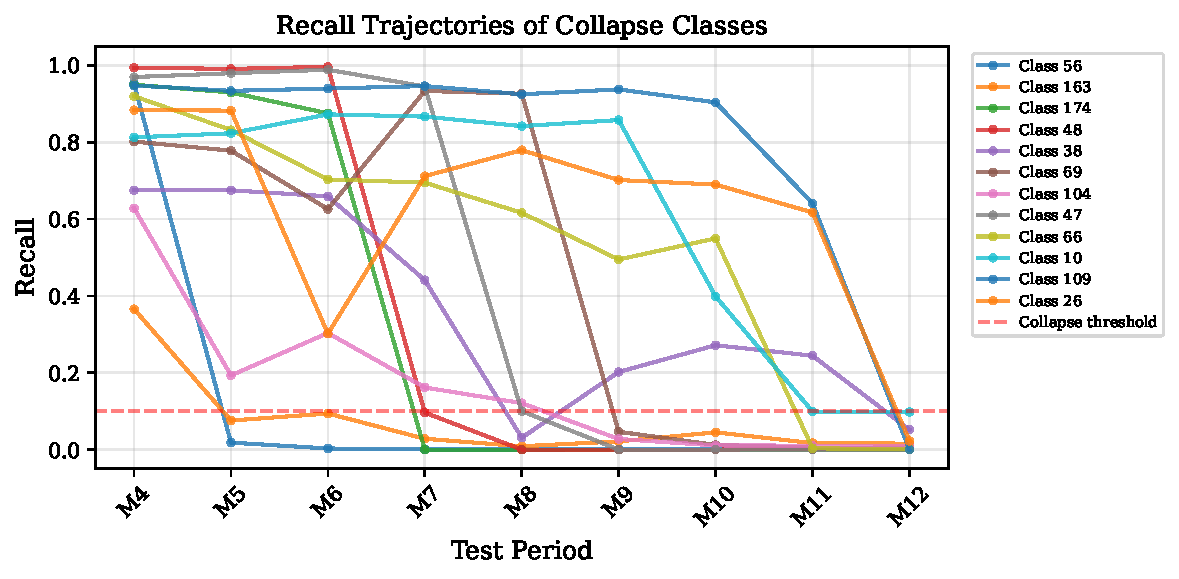
\includegraphics[width=\columnwidth]{fig_collapse_timeline.pdf}
\caption{Recall trajectories of 12 collapse classes on CESNET-TLS-Year22. Classes exhibit both abrupt collapse (\eg{}, class~56 at M5) and gradual decline (\eg{}, class~104 over M5--M9). By M12, all 12 classes fall below the 0.1 recall threshold (dashed line).}
\label{fig:collapse_timeline}
\end{figure}

Figure~\ref{fig:collapse_timeline} shows the recall trajectory of 12 classes that collapse below 0.1 recall by month 12.
The collapses follow two distinct temporal patterns:
\begin{itemize}
  \item \textbf{Abrupt collapse}: Recall drops sharply within one month (\eg{}, class~56 drops from 0.95 to 0.02 at M5 due to certificate rotation).
  \item \textbf{Gradual collapse}: Recall decays steadily over several months (\eg{}, class~104 declines from 0.63 to 0.01 over M3--M9).
\end{itemize}

% Absorber pattern
Crucially, these collapses are not random---each victim class has a \textit{primary absorber}: a dominant class that captures the majority of the victim's mispredictions.
Table~\ref{tab:absorber_pairs} lists the 12 collapse classes and their absorbers, with confusion rates ranging from 21\% to 77\%.

\begin{table}[t]
\centering
\caption{Absorber-collapse pairs at M-2022-12. Each collapsed class has a dominant absorber that captures the majority of its mispredictions.}
\label{tab:absorber_pairs}
\small
\begin{tabular}{@{}cccccc@{}}
\toprule
Victim & Absorber & Confusion & Victim & Pattern & First \\
Class  & Class    & Rate      & Recall & Type    & Collapse \\
\midrule
56  & 96  & 25.2\% & 0.000 & abrupt  & M5 \\
163 & 46  & 41.8\% & 0.015 & gradual & M5 \\
174 & 2   & 29.2\% & 0.000 & abrupt  & M7 \\
48  & 14  & 39.0\% & 0.001 & abrupt  & M7 \\
38  & 45  & 46.1\% & 0.052 & abrupt  & M8 \\
69  & 105 & 37.7\% & 0.005 & abrupt  & M9 \\
104 & 2   & 21.2\% & 0.010 & gradual & M9 \\
47  & 5   & 45.1\% & 0.000 & gradual & M11 \\
66  & 71  & 13.9\% & 0.001 & abrupt  & M11 \\
10  & 156 & 36.5\% & 0.098 & gradual & M11 \\
109 & 71  & 24.9\% & 0.000 & abrupt  & M12 \\
26  & 13  & ---    & 0.019 & ---     & --- \\
\bottomrule
\end{tabular}
\end{table}

\subsection{Two Mechanisms of Collapse}
\label{sec:mechanisms}

By comparing the Fisher discriminant ratio (inter-class distance / sum of intra-class spreads) between victim-absorber pairs at M4 (pre-collapse) and M12 (post-collapse), we identify two distinct mechanisms:

\begin{itemize}
  \item \textbf{Feature drift} (classes 56, 174, 38, 163): The victim's feature distribution physically shifts toward the absorber in feature space. Fisher ratio decreases 14--49\% from M4 to M12 (\eg{}, class~174$\to$2: Fisher drops from 0.635 to 0.326). This occurs when application updates cause the victim's traffic patterns to resemble the absorber's.
  \item \textbf{Boundary shift} (classes 48, 104): The inter-class distance remains stable or even increases (Fisher ratio rises 30\%), yet the classifier still absorbs the victim. This suggests the decision boundary shifts due to changes in other classes' distributions, indirectly pushing the victim onto the absorber's side.
\end{itemize}

The two mechanisms have implications for repair: feature-drift collapse can be addressed by re-anchoring the victim's prototype, while boundary-shift collapse requires recalibrating the decision boundary across multiple classes simultaneously. \ours{}'s combination of targeted fine-tuning and source replay addresses both mechanisms.

\subsection{Why General TTA Methods Fail}
\label{sec:tta_eval}

We evaluate seven TTA methods from computer vision on the same setup.
Table~\ref{tab:tta_baselines} reports results at three time points.
All methods maintain stable-class F1 near 0.90 but provide \textit{no improvement} on collapse classes.

\begin{table}[t]
\centering
\caption{TTA baselines on CESNET-TLS-Year22. All TTA methods fail to address class collapse. \ours{} uses strict evaluation (queried excluded, 3 seeds).}
\label{tab:tta_baselines}
\small
\begin{tabular}{@{}l ccc ccc@{}}
\toprule
& \multicolumn{3}{c}{Collapse-Class F1} & \multicolumn{3}{c}{Overall Macro-F1} \\
\cmidrule(lr){2-4} \cmidrule(lr){5-7}
Method & M7 & M9 & M12 & M7 & M9 & M12 \\
\midrule
Static     & .023 & .055 & .028 & .740 & .691 & .629 \\
Tent       & .025 & .053 & .026 & .742 & .691 & .631 \\
EATA       & .023 & .055 & .028 & .740 & .691 & .629 \\
SAR        & .024 & .054 & .026 & .740 & .690 & .629 \\
CoTTA      & .024 & .054 & .027 & .741 & .691 & .629 \\
NOTE       & .024 & .055 & .027 & .740 & .691 & .630 \\
\midrule
\textbf{\ours{}}$^\dagger$ & \textbf{.456} & \textbf{.159} & \textbf{.238} & \textbf{.750} & \textbf{.722} & \textbf{.674} \\
\bottomrule
\multicolumn{7}{l}{\footnotesize $^\dagger$Margin selection, $B$=1000, auto-discovered absorbers, strict eval.}
\end{tabular}
\end{table}

The failure of TTA methods is explained by their design: entropy minimization (Tent, SAR) and pseudo-label refinement (CoTTA, NOTE) optimize global prediction confidence, not class-specific confusion patterns.
When an absorber class confidently captures a victim's predictions, entropy is \textit{low} (the model is confidently wrong), so entropy-based adaptation sees no signal to correct.


% ============================================================
\section{Method: Collapse-Aware Active Repair}
\label{sec:method}

% Overview
\ours{} operates on a frozen encoder and repairs only the classification head, using three complementary mechanisms.
Algorithm~\ref{alg:care} summarizes the procedure.

\subsection{Absorber-Victim Identification}

Given a reference period with labels, we compute the confusion matrix and identify pairs where a victim class $v$ has a disproportionate fraction of its predictions redirected to an absorber class $a$:
\begin{equation}
  \text{confusion}(v \to a) = \frac{|\{x : y(x)=v, \hat{y}(x)=a\}|}{|\{x : y(x)=v\}|} > \tau_{\text{conf}}
\end{equation}

\subsection{Active Sample Selection}

From the target period, we select a budget $B$ of samples for labeling. We evaluate multiple strategies (\S\ref{sec:al_baselines}) and find that \textit{margin sampling}---selecting samples with the smallest gap between top-two logits---is the most effective deployable strategy. These boundary samples naturally concentrate on absorber-victim decision boundaries where labels are most informative.
When absorber identity is known, \textit{absorber-margin} restricts selection to absorber-predicted samples, further improving collapse repair at the cost of requiring oracle or auto-discovered absorber lists (\S\ref{sec:auto_absorber}).

\subsection{Head Fine-Tuning with Source Replay}

We fine-tune only the classification head $h_\theta$ using the selected target labels combined with $k$ samples per class from the reference period (source replay):
\begin{equation}
  \mathcal{L}_{\text{ft}} = \frac{1}{|D_{\text{target}} \cup D_{\text{replay}}|} \sum_{(x,y)} \ell_{\text{CE}}(h_\theta(f(x)), y)
\end{equation}
where $f(\cdot)$ is the frozen encoder.
Source replay prevents the head from overfitting to the small target sample and forgetting stable classes.

\subsection{Knowledge Distillation}

On replay samples, we add a KL-divergence loss~\cite{hinton2015distilling} between the updated head $h_\theta$ and the original (frozen) head $h_{\theta_0}$:
\begin{equation}
  \mathcal{L}_{\text{KD}} = \frac{1}{|D_{\text{replay}}|} \sum_{x \in D_{\text{replay}}} D_{\text{KL}}\!\left(\sigma\!\left(\frac{h_{\theta_0}(f(x))}{T}\right) \,\Big\|\, \sigma\!\left(\frac{h_\theta(f(x))}{T}\right)\right)
\end{equation}
where $T$ is the temperature and $\sigma$ is softmax.
Distillation ensures that repairing collapsed classes does not shift the classifier's behavior on classes where it already performs well.

\subsection{Combined Objective}

\begin{equation}
  \mathcal{L} = \mathcal{L}_{\text{ft}} + \lambda_{\text{KD}} \cdot \mathcal{L}_{\text{KD}}
\end{equation}

\begin{algorithm}[t]
\caption{\ours{}: Collapse-Aware Active Repair}
\label{alg:care}
\begin{algorithmic}[1]
\REQUIRE Source model $f, h_{\theta_0}$; class prototypes $\mathbf{P}$; target data $D_{\text{tgt}}$ (unlabeled); budget $B$
\STATE \textbf{Trigger:} Monitor mean confidence; activate if $\Delta_{\text{conf}} < \tau$
\STATE Compute features $\{f(x) : x \in D_{\text{tgt}}\}$ and logits
\STATE Select $B$ samples via margin sampling; query labels
\STATE Generate $D_{\text{replay}}$: $k$ synthetic samples per class from $\mathbf{P}$ + noise
\STATE Initialize $h_\theta \leftarrow h_{\theta_0}$
\FOR{epoch $= 1, \ldots, E$}
  \STATE Sample minibatch from $D_{\text{target}} \cup D_{\text{replay}}$
  \STATE $\mathcal{L} \leftarrow \mathcal{L}_{\text{ft}} + \lambda_{\text{KD}} \cdot \mathcal{L}_{\text{KD}}$
  \STATE Update $\theta$ via gradient descent on $\mathcal{L}$
\ENDFOR
\RETURN Updated classifier $h_\theta$
\end{algorithmic}
\end{algorithm}


% ============================================================
\section{Experiments}
\label{sec:experiments}

\subsection{Experimental Setup}

\textbf{Datasets.}
We use CESNET-TLS-Year22~\cite{hynek2024cesnet} (178 classes, 12 months, TLS traffic) and CESNET-QUIC22~\cite{luxemburk2023quic} (102 classes, 4 weeks, QUIC traffic).
For TLS22, we train on M-2022-3 (March 2022) and evaluate at M7, M9, M11, and M12.
For QUIC22, we train on W44 and evaluate at W46 and W47.

\textbf{Baselines.}
We compare against: (1)~Static (no adaptation), (2)~BN-Adapt~\cite{schneider2020bn}, (3)~Tent~\cite{wang2021tent}, (4)~EATA~\cite{niu2022eata}, (5)~CoTTA~\cite{wang2022cotta}, (6)~SAR~\cite{niu2023sar}, (7)~NOTE~\cite{gong2022note}, and (8)~CAPS, a prototype-based online adaptation method that maintains per-class prototypes and updates them using high-confidence predictions without labels.

\textbf{Evaluation protocol.}
All \ours{} results use \textit{strict evaluation}: the labeled samples selected for fine-tuning are \textit{excluded} from the test set before computing metrics, eliminating any possibility of train-test leakage.
Results are averaged over 5 random seeds with standard deviations reported.

\textbf{Metrics.}
Overall macro-F1, collapse-class macro-F1 (averaged over classes with recall $<0.1$ in the static model), stable-class macro-F1 (averaged over 20 consistently high-recall classes), and the number of collapsed classes (recall $< 0.1$).

\textbf{\ours{} configuration.}
Budget $B=1000$, margin-based selection (no absorber knowledge required), replay with $k=5$ samples per class from stable and absorber classes, target repeat factor 2, distillation weight $\lambda_{\text{KD}}=0.5$, temperature $T=2.0$, head fine-tuning learning rate $10^{-3}$, 30 epochs.

\subsection{Main Results}

Table~\ref{tab:main_results} presents the main comparison at M-2022-12 (the most challenging time point, 9 months after training).

\begin{table}[t]
\centering
\caption{Main results on CESNET-TLS-Year22 at M-2022-12. \ours{} results use strict evaluation (queried samples excluded) averaged over 5 seeds.}
\label{tab:main_results}
\small
\begin{tabular}{@{}l cccc@{}}
\toprule
Method & Macro-F1 & Collapse F1 & Stable F1 & Collapsed \\
\midrule
\multicolumn{5}{l}{\textit{No labeled target data:}} \\
Static          & .629 & .028 & .903 & 12 \\
Tent            & .631 & .026 & .903 & 12 \\
EATA            & .629 & .028 & .903 & 12 \\
SAR             & .629 & .026 & .901 & 11 \\
CoTTA           & .629 & .027 & .903 & 12 \\
NOTE            & .630 & .027 & .902 & 12 \\
\midrule
\multicolumn{5}{l}{\textit{Active learning with 1{,}000 labels + CARE components:}} \\
Entropy         & .601$\pm$.004 & .074$\pm$.013 & .883 & 9.8 \\
Coreset         & .621$\pm$.005 & .124$\pm$.010 & .877 & 8.8 \\
Random          & .655$\pm$.005 & .179$\pm$.030 & .890 & 8.0 \\
\textbf{Margin (\ours{})} & \textbf{.673$\pm$.001} & \textbf{.233$\pm$.002} & .886 & \textbf{5.2} \\
\bottomrule
\multicolumn{5}{l}{\footnotesize All active methods use CARE components (replay + distillation).}\\
\multicolumn{5}{l}{\footnotesize Entropy and coreset perform \textit{worse} than Static on macro-F1.}
\end{tabular}
\end{table}

\subsection{Per-Class Recovery Analysis}

Table~\ref{tab:per_class} illustrates per-class repair outcomes when oracle absorber knowledge is available (absorber-margin strategy), representing the upper bound of \ours{}'s repair capability.

\begin{table}[t]
\centering
\caption{Per-class recovery at M-2022-12 (absorber-margin, $B$=1000, oracle absorber list). This represents the diagnostic upper bound; the deployable margin strategy achieves aggregate collapse F1 of $0.233{\pm}0.002$.}
\label{tab:per_class}
\small
\begin{tabular}{@{}c cc cc l@{}}
\toprule
Class & \multicolumn{2}{c}{Recall} & \multicolumn{2}{c}{F1} & Outcome \\
\cmidrule(lr){2-3} \cmidrule(lr){4-5}
      & Before & After & Before & After & \\
\midrule
48  & 0.001 & \textbf{0.913} & 0.002 & 0.881 & Full recovery \\
56  & 0.000 & \textbf{0.733} & 0.001 & 0.799 & Full recovery \\
47  & 0.000 & \textbf{0.699} & 0.000 & 0.637 & Full recovery \\
104 & 0.010 & \textbf{0.624} & 0.016 & 0.607 & Substantial \\
10  & 0.098 & \textbf{0.623} & 0.162 & 0.662 & Substantial \\
38  & 0.052 & \textbf{0.534} & 0.090 & 0.518 & Substantial \\
163 & 0.016 & \textbf{0.455} & 0.026 & 0.446 & Moderate \\
66  & 0.001 & \textbf{0.355} & 0.002 & 0.270 & Partial \\
174 & 0.000 & 0.274 & 0.000 & 0.230 & Partial \\
\midrule
26  & 0.022 & 0.051 & 0.025 & 0.065 & Failed \\
69  & 0.005 & 0.000 & 0.008 & 0.000 & Failed \\
109 & 0.000 & 0.000 & 0.000 & 0.000 & Failed \\
\bottomrule
\end{tabular}
\end{table}

Nine of 12 collapsed classes recover above the 0.1 recall threshold, with five exceeding 0.62 recall. The three failures share a common pattern: extremely low support or diffuse confusion without a clear absorber target.

\subsection{Ablation Study}

Table~\ref{tab:ablation} validates the necessity of each component.
All ablations use the absorber-margin strategy with budget $B=1000$ to ensure controlled comparison; only the component under test is varied.

\begin{table}[t]
\centering
\caption{Ablation study at M-2022-12 (margin selection, $B$=1000, strict evaluation, 5 seeds). Each component plays a distinct, non-redundant role.}
\label{tab:ablation}
\small
\begin{tabular}{@{}l cccc@{}}
\toprule
Configuration & Macro-F1 & Collapse F1 & Stable F1 & Collapsed \\
\midrule
Static (no repair)      & .629 & .028 & \textbf{.903} & 12 \\
FT only                 & .638$\pm$.001 & .134$\pm$.001 & .838 & 7.0 \\
FT + Replay             & .620$\pm$.001 & .224$\pm$.002 & .840 & 5.0 \\
FT + Distill            & .670$\pm$.000 & .152$\pm$.007 & .887 & 7.8 \\
\midrule
\textbf{\ours{} (Full)} & \textbf{.673$\pm$.001} & \textbf{.233$\pm$.002} & .885 & \textbf{5.2} \\
\bottomrule
\end{tabular}
\end{table}

Key findings:
\begin{itemize}
  \item \textbf{FT only}: Repairs collapse classes (F1: .028$\to$.134) but severely damages stable classes (.903$\to$.838).
  \item \textbf{+ Replay}: Improves collapse repair (.134$\to$.224) but does not protect stable classes (.840).
  \item \textbf{+ Distill}: Best stable-class preservation (.887, close to Static), but limited collapse repair (.152).
  \item \textbf{Full \ours{}}: Combines replay's collapse repair with distillation's stable protection---the only configuration that simultaneously improves collapse F1 and maintains stable F1 above 0.88.
\end{itemize}

\begin{figure}[t]
\centering
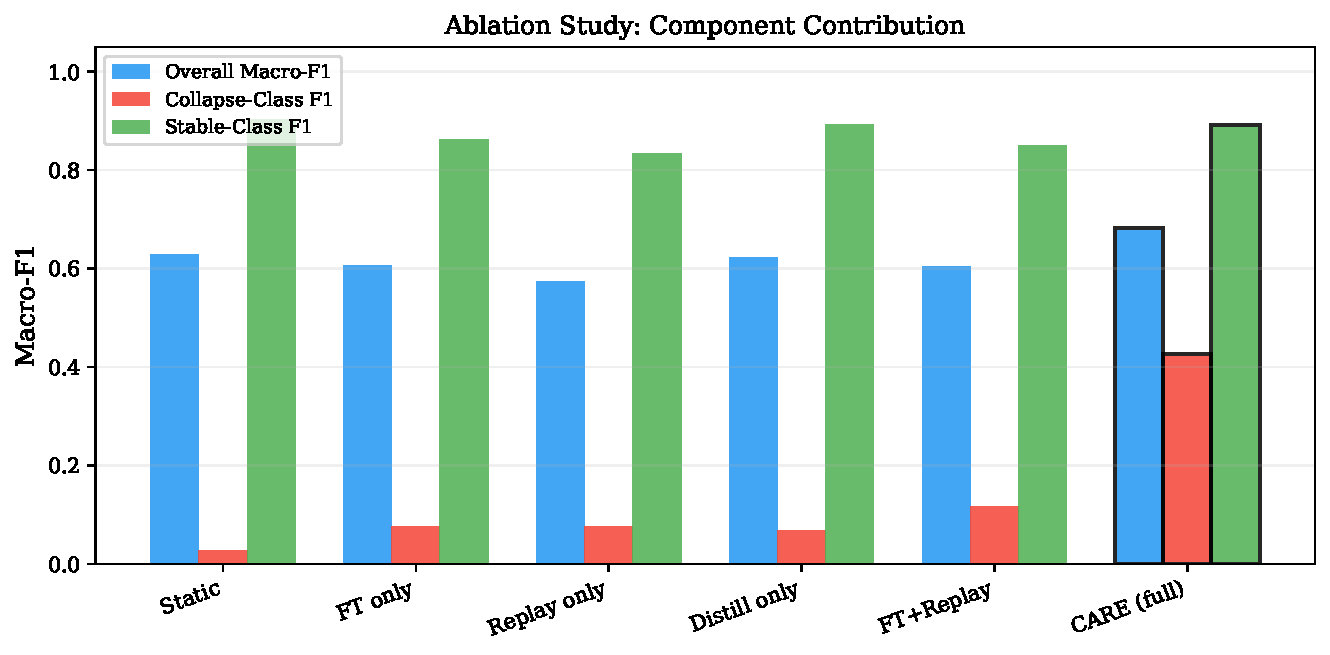
\includegraphics[width=\columnwidth]{fig_ablation_bar.pdf}
\caption{Ablation study visualization. Only the full \ours{} method (rightmost) simultaneously improves collapse-class F1 (red) while maintaining stable-class F1 (green).}
\label{fig:ablation_bar}
\end{figure}

\begin{figure}[t]
\centering
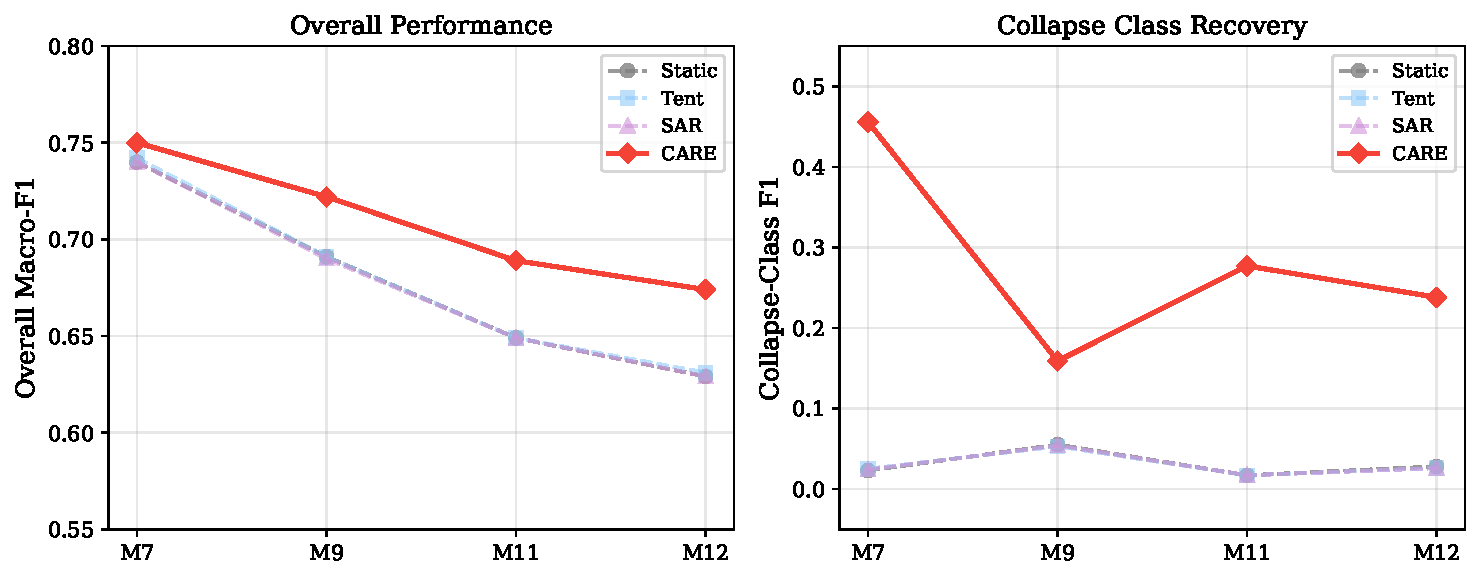
\includegraphics[width=\columnwidth]{fig_tta_failure.pdf}
\caption{Overall macro-F1 across time points. All TTA baselines track Static closely. \ours{} provides increasing benefit as drift severity grows.}
\label{fig:tta_failure}
\end{figure}

\subsection{Active Learning Baseline Comparison}
\label{sec:al_baselines}

A natural question is whether standard active learning (AL) strategies~\cite{settles2009active} suffice for collapse repair. Table~\ref{tab:main_results} includes entropy sampling and greedy coreset~\cite{sener2018coreset} as AL baselines, both using the same CARE components (replay + distillation) to isolate the effect of selection strategy.

Both standard AL methods perform \textit{worse} than the static baseline on macro-F1: entropy achieves 0.601 (vs.\ Static 0.629) and coreset achieves 0.621. The reason is that these methods select globally uncertain or representative samples, which are dominated by high-traffic classes. Entropy sampling is particularly harmful because absorber classes produce \textit{confident} mispredictions (low entropy), so entropy-based selection systematically avoids the collapse boundary---exactly where labels are most needed.

Margin sampling succeeds because it targets samples where the top-two predictions are close, which naturally concentrates on absorber-victim decision boundaries. This confirms that class collapse is not a generic active learning problem but requires selection strategies aware of the confusion structure.

\subsection{Automatic Absorber Discovery}
\label{sec:auto_absorber}

For deployment, absorber-victim pairs must be discovered without oracle knowledge of the target period.
We propose using a \textit{probe period}: running the static model on the immediately preceding period (\eg{}, M11 for target M12) and identifying classes with recall $<0.1$ as collapse candidates and their top false-positive receivers as absorbers.

Table~\ref{tab:auto_absorber} compares oracle vs.\ auto-discovered absorber lists with the absorber-margin strategy.

\begin{table}[t]
\centering
\caption{Oracle vs.\ auto-discovered absorber lists (absorber-margin, $B$=1000, 5 seeds).}
\label{tab:auto_absorber}
\small
\begin{tabular}{@{}l ccc@{}}
\toprule
Absorber Source & Macro-F1 & Collapse F1 & Collapsed \\
\midrule
Oracle (M12 ground truth) & .657$\pm$.002 & .377$\pm$.008 & 3.0 \\
Auto (M11$\to$M12) & .649$\pm$.002 & .289$\pm$.001 & 5.0 \\
Margin (no absorber info) & \textbf{.673$\pm$.001} & .233$\pm$.002 & 5.2 \\
\bottomrule
\end{tabular}
\end{table}

Auto-discovered absorbers from M11 are partially effective (collapse F1: 0.289 vs.\ oracle 0.377), confirming that absorber relationships evolve over time. Notably, the margin strategy---which uses \textit{no} absorber information---achieves the highest macro-F1 (0.673) because it is not restricted to absorber-predicted samples. We therefore recommend margin as the default deployable strategy.

\subsection{Multi-Period Analysis}

Table~\ref{tab:multiperiod} shows \ours{}'s effectiveness across four time points with auto-discovered absorbers.

\begin{table}[t]
\centering
\caption{Multi-period CARE results (margin, $B$=1000, auto-discovery, 3 seeds).}
\label{tab:multiperiod}
\small
\begin{tabular}{@{}l cc cc c@{}}
\toprule
& \multicolumn{2}{c}{Static} & \multicolumn{2}{c}{\ours{}} & \\
\cmidrule(lr){2-3} \cmidrule(lr){4-5}
Period & Macro & Collapse & Macro & Collapse & $\Delta$Macro \\
\midrule
M7 (light)  & .740 & .023 & .750$\pm$.001 & .456 & +.010 \\
M9 (medium) & .691 & .055 & .722$\pm$.001 & .159 & +.031 \\
M11 (heavy) & .649 & .017 & .689$\pm$.001 & .277 & +.040 \\
M12 (severe)& .629 & .031 & .674$\pm$.002 & .238 & +.045 \\
\bottomrule
\end{tabular}
\end{table}

\ours{} is effective at all drift levels, with increasing benefit as drift severity grows (M7: +0.010; M12: +0.045). Collapse repair is most successful at M7, where the absorber-victim separation in feature space is still partially intact ($\text{collapse F1}=0.456$).

\subsection{Prototype-Based Replay}
\label{sec:proto_replay}

Standard \ours{} requires storing reference-period samples for replay, which may be infeasible in privacy-sensitive deployments. We propose \textit{prototype replay}: generating synthetic features from stored class prototypes (mean feature vectors) with per-class Gaussian noise estimated from reference statistics. This requires storing only prototypes (178$\times$256 floats = 178~KB) instead of raw training data.

\begin{table}[t]
\centering
\caption{Real vs.\ prototype replay (margin, $B$=1000, 3 seeds).}
\label{tab:proto_replay}
\small
\begin{tabular}{@{}l ccc@{}}
\toprule
Replay Mode & Macro-F1 & Collapse F1 & Stable F1 \\
\midrule
Real (source samples) & .673$\pm$.001 & .231$\pm$.001 & .884$\pm$.003 \\
Prototype (exemplar-free) & .664$\pm$.001 & .219$\pm$.003 & .878$\pm$.002 \\
\midrule
\multicolumn{4}{l}{Performance gap: $<$1\% macro-F1} \\
\bottomrule
\end{tabular}
\end{table}

Prototype replay achieves 98.7\% of real replay's macro-F1 (0.664 vs.\ 0.673), demonstrating that \ours{} can operate in an exemplar-free setting with minimal performance loss.

\subsection{Architecture Independence}

To verify that \ours{} is not architecture-specific, we train a Transformer backbone~\cite{vaswani2017attention} (4-layer, 4-head, 256-dim) on the same data and apply CARE.

\begin{table}[t]
\centering
\caption{Architecture comparison (margin, $B$=1000, M-2022-12).}
\label{tab:arch}
\small
\begin{tabular}{@{}l cc cc@{}}
\toprule
& \multicolumn{2}{c}{Static} & \multicolumn{2}{c}{\ours{}} \\
\cmidrule(lr){2-3} \cmidrule(lr){4-5}
Backbone & Macro & Collapse & Macro & Collapse \\
\midrule
CNN & .629 & .028 & .673$\pm$.001 & .233$\pm$.002 \\
Transformer & .670 & .030 & \textbf{.767$\pm$.001} & \textbf{.401$\pm$.003} \\
\bottomrule
\end{tabular}
\end{table}

CARE improves both architectures consistently. The Transformer benefits more (macro +0.097 vs.\ +0.044), likely because its richer feature representations provide better material for head-only repair.

\subsection{Deployment Trigger}
\label{sec:trigger}

We propose monitoring mean prediction confidence as an unsupervised trigger for \ours{} activation. Across M4--M12, mean confidence decreases monotonically with drift severity. Setting a threshold of $\Delta_{\text{conf}} < -0.05$ (relative to the reference period) triggers at M9, when 10 classes have already collapsed. A more aggressive threshold ($-0.03$) triggers at M7 with 7 collapsed classes, enabling earlier intervention.

\subsection{Generalization to QUIC22}

On CESNET-QUIC22, concept drift is milder: the static model maintains macro-F1 of 0.719 at W-2022-47 with fewer severely collapsed classes. Under strict evaluation with auto-discovered absorbers (probe: W-2022-46, threshold 0.3), \ours{} with margin selection achieves macro-F1 of $0.718{\pm}0.003$---essentially unchanged from Static.
The collapse-class F1 improves modestly ($0.305\to0.413$), confirming that \ours{}'s benefit scales with collapse severity. When drift is mild, the method does no harm but provides limited gain, which is the expected behavior for a collapse-targeted repair framework.


% ============================================================
\section{Discussion}
\label{sec:discussion}

\textbf{Label cost.}
\ours{} requires 1{,}000 labeled samples per repair cycle---less than 0.3\% of a typical monthly test set.
In ISP deployment, this can be obtained through a few hours of DPI-based labeling on a monitored subnet, or via periodic manual verification of a stratified sample.

\textbf{Stable-class trade-off.}
Stable-class F1 decreases from 0.903 to 0.885 ($-$2.0\%).
The ablation shows each component's contribution: without replay and distillation, degradation is severe (0.838); adding distillation alone recovers most stability (0.887). The full method limits degradation to 2.0\%, an acceptable trade-off for recovering 7 collapsed classes.

\textbf{Deployability.}
\ours{} is designed for deployment without oracle knowledge:
(1)~absorber-victim pairs are discovered automatically from a probe period (\S\ref{sec:auto_absorber});
(2)~margin selection requires no absorber information and achieves the highest macro-F1;
(3)~prototype replay eliminates source data storage (\S\ref{sec:proto_replay});
(4)~a confidence-based trigger determines when repair is needed (\S\ref{sec:trigger}).
The complete pipeline requires only stored prototypes (178~KB) and a small labeled budget.

\textbf{Limitations.}
Three classes (26, 69, 109) remain collapsed after repair, suggesting \ours{} is most effective when the absorber-victim relationship is clear and the victim retains some discriminative features.
On QUIC22, where drift is mild, macro-F1 improvement is negligible.
\ours{} addresses \textit{existing} class collapse but does not handle emerging new classes---a complementary problem addressed by class-incremental methods such as CPN~\cite{cai2024cpn}.

\textbf{Week-10 data collection change.}
CESNET-TLS-Year22 has a known distribution shift at week 10 due to a flow exporter update~\cite{hynek2024cesnet}.
This affects all methods equally and does not invalidate comparative results.


% ============================================================
\section{Conclusion}
\label{sec:conclusion}

We identified and formalized the absorber-collapse pattern in encrypted traffic classifiers: a systematic failure mode where dominant classes absorb predictions from victim classes under concept drift.
We showed that both test-time adaptation methods and standard active learning strategies fail on this task, establishing class collapse as a distinct problem.
We proposed \ours{}, a deployable repair framework combining margin-based active selection, source replay, and knowledge distillation.
Under strict evaluation with 5 random seeds, \ours{} improves collapse-class F1 from 0.028 to $0.233{\pm}0.002$ and macro-F1 from 0.629 to $0.673{\pm}0.001$ using only 1{,}000 labels ($<$0.3\% of test data), with consistent gains across time points (M7--M12), architectures (CNN/Transformer), and an exemplar-free deployment mode via prototype replay.
The complete pipeline---automatic absorber discovery, confidence-based trigger, and targeted repair---operates without oracle knowledge, making \ours{} practical for real-world encrypted traffic monitoring.

% ============================================================
\bibliographystyle{IEEEtran}
\bibliography{references}

\end{document}
